\chapter{Isosurface extraction with Marching Cubes}

This chapter will present a method of isosurface extraction that is later used
in the programming project. First, basic definitions will be established and
rationale for generating graphics with volumetric data will be discussed.
Next, brief history and high level overview of Marching Cubes will be presented.
Technical details will follow with description of implementation on highly
parallel GPGPU systems with OpenCL.

\section{Definitions}

\begin{defn}[Density function]
\label{def:density function}
Scalar function
$\mathbb{R}^3\rightarrow\mathbb{R}$ or $\mathbb{R}^2\rightarrow\mathbb{R}$
that defines value of some magnitude in a continuous space. An example of such
function in 3D space is temperature defined in each point in the space. Height
on a flat map on the other hand is a density function in 2D space.
\end{defn}

\begin{defn}[Isosurface]
Surface in three-dimensional space that consists of points that have certain
value of \emph{density function}.
\end{defn}

\begin{defn}[Isovalue]
Certain value of density function which will be considered the surface. Points
in domain which density function value is below this value are considered to
lie below the surface and points which density function value is above this
value are considered to lie above the surface. Points which density function
value equals isovalue are considered to lie exactly on the isosurface.
\end{defn}

\section{Rationale for isosurface rendering}

There are many applications which yield data as a density function. Some of them
are listed below:
\begin{description}
	\item[CT\footnotemark scan.]\footnotetext{Computer Tomography}
		Result of such scan is a discrete lattice of points with certain
		values on vertices
	\item[Weather data]
		Weather data, especially coming from weather models consists of
		scalar values of various parameters (temperature, humidity, etc.)
		on earth's surface
	\item[Arbitrary mathematical function]
		It's often desirable to visualise mathematical function with
		multiple parameters on 2D and 3D plots. For example for
		educational purposes.
	\item[Procedural models]
		Surfaces expressed by density function may be a source of
		visually interesting models that could be hard to model by hand.
\end{description}

Interactive presentation of such data may be very helpful while working with
these applications. Ability to rotate, zoom and scale such surfaces may be
beneficial to understanding the data since human sight apparatus is naturally
well equipped to process 3D objects and images.

\section{Marching Cubes algorithm overview}
\subsection{History \parencite{mchist}}
Marching Cubes algorithm was invented in 1984 by William E. Lorensen and Harvey
E. Cline. While being employed by General Electric they attended a seminar by
GE's Medical Systems Business Group employee Carl Crawford. Mr Crawford
described capabilities of the upcoming rendering engine called \emph{Graphicon},
that rendered using polygons. He also challenged seminar attendees to find
interesting usages for the device. Within a day Lorenson and Cline devised an
algorithm that read volumetric medical data (essentially a density function) and
produced triangle mesh representing isosurface.

General Electric submitted a patent application for the algorithm on
June~5, 1985, which was granted on December~1, 1987 \parencite{mcpatent}.

Partly due to existence of this patent, another algorithm for isosurface
extraction called \emph{Marching Tetrahedra} was invented to give graphics
community method that is not encumbered by patents. \emph{Marching Tetrahedra}
also solves some ambiguities that are present in \emph{Marching Cubes}.

Patent on \emph{Marching Cubes} algorithm expired in 2005.

\subsection{Algorithm description \parencite{Lorensen:1987:MCH:37402.37422}}

Marching cubes algorithm divides space on which it operates into a discrete
lattice of cubes. For each cube, density function value is retrieved for each
vertex of the cube. Density function may be calculated from the position of the
vertex on the fly if it's defined as a mathematical function, or it may be
extracted from some external volumetric data source (e.g. result of CT scan).

Next, for each edge of the cube it's determine whether value at given vertex is
larger or smaller than requested isovalue. If the value on the vertex is smaller
than the threshold isovalue, vertex is below the surface. Otherwise it's above
it.

Being above or below the surface will be called the \emph{sign} of the vertex.
If vertices on the ends of given cube's edge are of different signes, than it's
certain that the surface crosses the edge.

For each cube, there are $2^8=256$ possible combinations of sings of the
vertices. Combination of the cube is called an \emph{index} of this cube.

When the index of the cube is known, pre-generated LUTs\footnote{Look-Up Tables}
are consulted to determine how many polygons and in what configuration should be
emitted for this cube.

Process is repeated for all cubes in the lattice emitted polygons are the output
of the algorithm.

\subsubsection{Cube indexing}

Operation on a single cube begins with evaluating density function on each
vertex of the cube.

Index of the vertex is calculated through operation described below
Figure~\ref{fig:mcnumbering}.

\begin{figure}
  \centerline{
   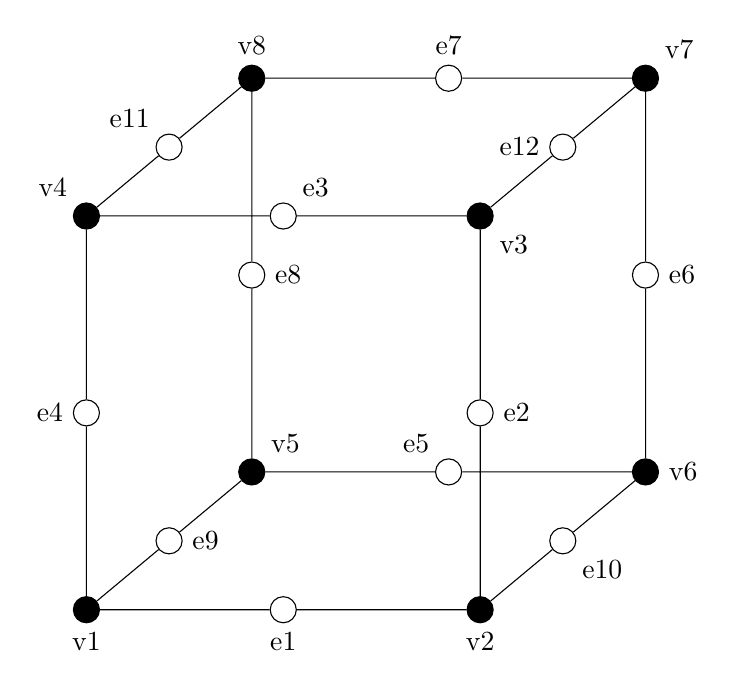
\begin{tikzpicture}[
  z={(-0.42cm,-0.35cm)}, scale=2.5,
  vert/.style={circle,draw=black,fill=black},
  edge/.style={circle,draw=black,fill=white}
]
 
  \node at (0,0,0) [vert,label=below:v1] (v1) {};
  \node at (1,0,0) [edge,label=below:e1] (e1) {};
  \node at (2,0,0) [vert,label=below:v2] (v2) {};
  \node at (2,1,0) [edge,label=right:e2] (e2) {};
  \node at (2,2,0) [vert,label=south east:v3] (v3) {};
  \node at (1,2,0) [edge,label=north east:e3] (e3) {};
  \node at (0,2,0) [vert,label=north west:v4] (v4) {};
  \node at (0,1,0) [edge,label=left:e4] (e4) {};
  \node at (0,0,-2) [vert,label=north east:v5] (v5) {};
  \node at (1,0,-2) [edge,label=north west:e5] (e5) {};
  \node at (2,0,-2) [vert,label=right:v6] (v6) {};
  \node at (2,1,-2) [edge,label=right:e6] (e6) {};
  \node at (2,2,-2) [vert,label=north east:v7] (v7) {};
  \node at (1,2,-2) [edge,label=above:e7] (e7) {};
  \node at (0,2,-2) [vert,label=above:v8] (v8) {};
  \node at (0,1,-2) [edge,label=right:e8] (e8) {};
  \node at (0,0,-1) [edge,label=right:e9] (e9) {};
  \node at (2,0,-1) [edge,label=south east:e10] (e10) {};
  \node at (2,2,-1) [edge,label=left:e12] (e12) {};
  \node at (0,2,-1) [edge,label=north west:e11] (e11) {};

  \draw
    (v1) -- (e1) -- (v2) -- (e2) -- (v3) -- (e3) -- (v4) -- (e4) -- (v1)
    (v5) -- (e5) -- (v6) -- (e6) -- (v7) -- (e7) -- (v8) -- (e8) -- (v5)
    (v1) -- (e9) -- (v5)
    (v2) -- (e10) -- (v6)
    (v4) -- (e11) -- (v8)
    (v3) -- (e12) -- (v7);
\end{tikzpicture}

  }
  \caption{
    Numbering of vertices and edges in Marching Cubes. Cube index is
    derived by concatenation of bits \texttt{index = v8|v7|v6|v5|v4|v3|v2|v1}
    where each \texttt{vi} is logical result (0 or 1) of operation of comparing
    density function value at \emph{i}-th vertex with threshold value
    (\texttt{value(i) > threshold}).
  }
  \label{fig:mcnumbering}
\end{figure}

\subsubsection{Emitting polygons}

When index of the cube is known, LUT is consulted that maps index to list of
edges on which vertex in given cube must be emitted.
\pagebreak
\begin{lstlisting}[caption={Index to edge list LUT. Notice that for indices 0
and 255 no geometry is emitted}]
unsigned char mcTriangleTable[256][16] = {
        {255, 255, 255, 255, 255, 255, 255, 255, 255, 255, 255, 255, 255, 255, 255, 255},
        {0, 8, 3, 255, 255, 255, 255, 255, 255, 255, 255, 255, 255, 255, 255, 255},
        ...
        {0, 3, 8, 255, 255, 255, 255, 255, 255, 255, 255, 255, 255, 255, 255, 255},
        {255, 255, 255, 255, 255, 255, 255, 255, 255, 255, 255, 255, 255, 255, 255, 255}
};
\end{lstlisting}

For each edge on the list vertex is emitted between its two ends in place
proportional to the linear interpolation of density function at the vertices.

Each three vertices form a polygon. In the listing above, value 255 marks an end
of the list for given index.

Next, each polygon is saved in a list for later usage, or directly fed to
rendering device.


\begin{figure}
  \centerline{
    \begin{tikzpicture}[z={(-0.58cm,-0.28cm)}, scale=1.5]
    \input{chapters/marchingcubes/cases.tex}
    \end{tikzpicture}
  }
  \caption{
    All cases in traditional Marching cubes algorithm. Vertices with density
    function above threshold value have black circles on them. Symmetries,
    rotations, and complementary cases (with exception of cases 0 and 255) were
    omitted for brevity.
  }
  \label{fig:mccases}
\end{figure}

\section{Implementation on GPU with OpenCL}
\subsection{Parallel prefix sum operation}
